\sectionframe{Minimal Reproducing Model}

\section{Minimal Reproducing Model}

\begin{frame}{Approach for Reproducing the Behaviour}
    \vspace{-1em}
    \begin{columns}
        \begin{column}{1 \textwidth}
            Idea:
            Try to mimic the evolution of the model function under parameter variation

            \vspace{-2.0em}
            \begin{figure}
                \centering
                \subfloat[Directions]{
                    \includegraphics[width=0.6 \textheight]{99_Yunus/2D_Period_Zoomed_EffectsSingle/result.png}
                }
                \subfloat[Evolution for Parameter $E_0$]{
                    \includegraphics[width=0.6 \textheight]{99_Yunus/ParameterEffects/E0/illustration.png}
                }
                \subfloat[Evolution for Parameter $\chi_0$]{
                    \includegraphics[width=0.6 \textheight]{99_Yunus/ParameterEffects/hi/illustration.png}
                }
                \caption*{Effects of the individual parameters on the function of the original model}
            \end{figure}
        \end{column}
    \end{columns}
\end{frame}

\begin{frame}{Approach for Reproducing the Behavior: Wishlist}
    Characteristics we want to keep:
    \begin{itemize}
        \item Symmetry
        \item Branches $f_{\A}$ and $f_{\C}$ move up
        \item The values at the left border of branches $f_{\B}$ and $f_{\D}$ move down
    \end{itemize}

    \vspace{2em}
    Characteristics we want to leave behind if possible:
    \begin{itemize}
        \item Borders between branch domains move
        \item Cubic shape of branches $f_{\B}$ and $f_{\D}$
        \item Other minimal changes
    \end{itemize}
\end{frame}

\begin{frame}{Path to the Reproducing Model}
    \begin{columns}
        \begin{column}{.5 \textwidth}
            Different Models
            \begin{itemize}
                \item Linear branches
                \item Quadratic branches
            \end{itemize}

            \vspace{2em}
            With different
            \begin{itemize}
                \item sets of fixed parameters
                \item sets of variable parameters
                \item values of the fixed parameters
            \end{itemize}
        \end{column}
        \begin{column}{.5 \textwidth}
            \vspace{-4em}
            \begin{figure}
                \centering
                \subfloat{\includegraphics[height=.4 \textheight]{20_Quadratic_mod2pi/First_Find/2D_Period_Heureka/result.png}}
                \qquad
                \subfloat{\includegraphics[height=.4 \textheight]{21_011_Quadratic_2aR1bR_centered/2D_Period_Selected/result.png}}
                \\
                \subfloat{\includegraphics[height=.4 \textheight]{21_012_Quadratic_2aR1bR_mirror/2D_Period_Whole/result.png}}
                \qquad
                \subfloat{\includegraphics[height=.4 \textheight]{40_Quadratic_fittingR/2D_Period_Whole/result.png}}
            \end{figure}
        \end{column}
    \end{columns}
\end{frame}

\begin{frame}{Definition of Minimal Reproducing Model (1/2)}
    \vspace{-3.0em}
    \begin{align}
        x \mapsto f(x) \mod 1
    \end{align}

    \begin{align}
        f(x) & = \begin{cases}
                     g(x)                                        & \text{ if } x < \frac{1}{2} \\
                     g\left(x - \frac{1}{2}\right) + \frac{1}{2} & \text{ else}
                 \end{cases}
    \end{align}

    \begin{align}
        g(x) & = \begin{cases}
                     l(x) = a_L \cdot x^2 + b_L \cdot x + c_L & \text{ if } x < \frac{1}{4} \\
                     r(x) = b_R \cdot x + c_R                 & \text{ else}
                 \end{cases}
    \end{align}
\end{frame}

\begin{frame}{Definition of Minimal Reproducing Model (2/2)}
    \vspace{-1em}
    \begin{columns}
        \begin{column}{.7 \textwidth}
            Fixed parameters:
            \begin{align*}
                a_L = 4, b_L = -\frac{1}{2}
            \end{align*}

            Variable parameters
            \begin{align*}
                 & c_L, b_R, c_R                                                    \\
                \text{where} \qquad
                 & c_L = p_y,                                                       \\
                 & b_R = 4 \cdot (B - A), c_R = 2A - B                              \\
                \text {and} \qquad
                 & A = p_x, \text{and } B = \frac{1}{2} + \epsilon \text{ is fixed}
            \end{align*}

            $A$ and $B$ are intermediated parameters for modeling the values of the left ($A$) and right ($B$) borders of $r(x)$
        \end{column}
        \begin{column}{.3 \textwidth}
            \begin{figure}
                \centering
                \includegraphics[height=.5 \textheight]{60_MinimalRepr/ParameterEffects/AB/illustration.png}
                \caption*{Illustration of the parameters $A$ and $B$}
            \end{figure}
        \end{column}
    \end{columns}
\end{frame}

\begin{frame}{Minimal Reproducing Model Parameter Effects}
    \vspace{-1.0em}
    \begin{figure}
        \centering
        \subfloat[Effect of $p_x$]{\includegraphics[height=0.6\textheight]{60_MinimalRepr/ParameterEffects/p_x/illustration.png}}
        \subfloat[Effect of $p_y$]{\includegraphics[height=0.6\textheight]{60_MinimalRepr/ParameterEffects/p_y/illustration.png}}
        \caption*{Effects of the Individual Parameters on the Function of the Minimal Reproducing Model}
    \end{figure}
\end{frame}

\begin{frame}{Minimal Reproducing Model Dynamics}
    \vspace{-1.0em}
    \begin{figure}
        \centering
        %    \subfloat[Full Model]{\includegraphics[height=0.6\textheight]{60_MinimalRepr/2D_Period_Whole_onlyP16_CDE/result.png}}
        %    \subfloat[Halved Model]{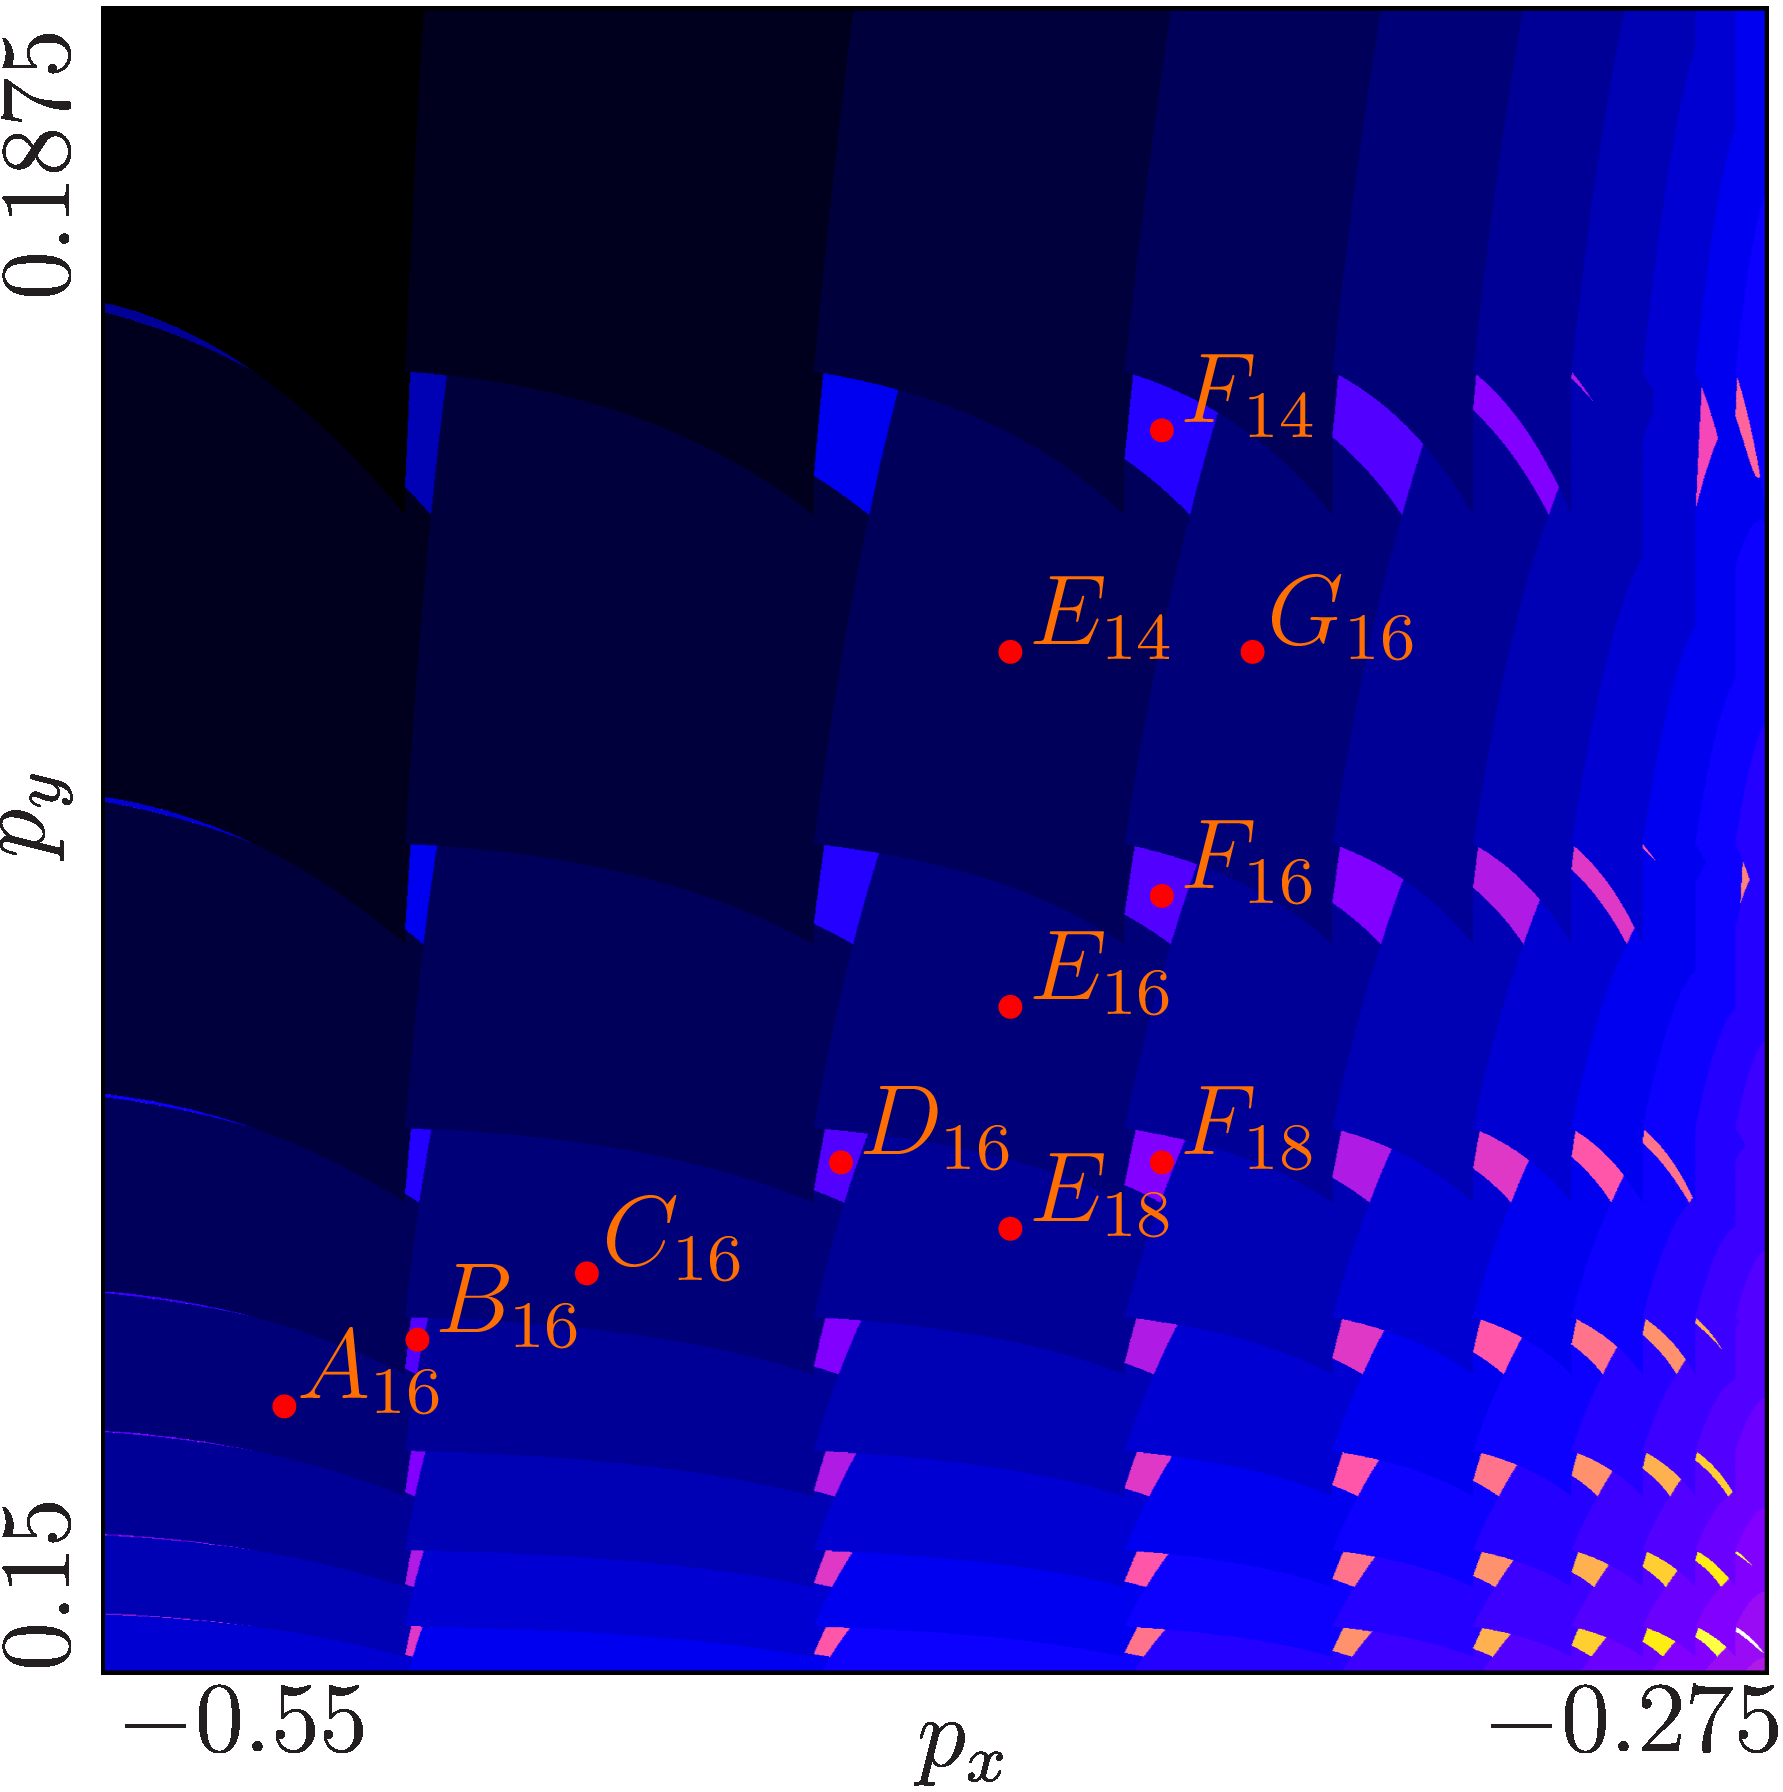
\includegraphics[height=0.6\textheight]{60_MinimalRepr/2D_Period_Whole_onlyP16_CDE/result-halved.png}}
        %    \caption{2D Scans of Periods of Minimal Reproducing Model}
        \subfloat[Periods]{ \includegraphics[height=.6 \textheight]{60_MinimalRepr/2D_Period_Whole_onlyP16_CDE/result.png} }
        \subfloat[Period Regions]{ \includegraphics[height=.6 \textheight]{60_MinimalRepr/2D_Regions_Whole/Manual/Chain16/result.png} }
        \caption*{2D scans of the minimal reproducing model}
    \end{figure}
\end{frame}

\begin{frame}{Minimal Reproducing Model Dynamics}
    \begin{columns}
        \begin{column}{.9 \textwidth}
            \vspace{-2em}
            \begin{figure}
                \centering
                \subfloat[$C_{16}$: Period 16, $\Cycle{\A^6\B^2\C^6\D^2}$]{
                    \includegraphics[height=0.5\textheight]{60_MinimalRepr/Cobweb_C16/result.png}
                }
                \subfloat[$D_{16}$: Period 16, $\Cycle{\A^6\B^2\C^7\D^3}$ and $\Cycle{\A^7\B^3\C^6\D^2}$]{
                    \includegraphics[height=0.5\textheight]{60_MinimalRepr/Cobweb_D16/result.png}
                }
                \subfloat[$E_{16}$: Period 16, $\Cycle{\A^7\B^3\C^7\D^3}$]{
                    \includegraphics[height=0.5\textheight]{60_MinimalRepr/Cobweb_E16/result.png}
                }
                \caption*{Cobwebs}
            \end{figure}
        \end{column}
        \begin{column}{.2 \textwidth}
            \vspace{-4em}
            \begin{center}
                \hspace{-2em}
                \includegraphics[height=0.3 \textheight]{60_MinimalRepr/2D_Period_Whole_onlyP16_CDE/result.png}
            \end{center}
        \end{column}
    \end{columns}
\end{frame}

\begin{frame}{Parameter Regions in Minimal Reproducing Model}
    \begin{itemize}
        \item ``Type A'': At points $C_{16}$ and $E_{16}$ in 2D scan
              \begin{itemize}
                  \item One cycle
                  \item Symmetrical
                  \item Example at point $C_{16}$: $\Cycle{\A^6\B^2\C^6\D^2}$
                  \item Example at point $E_{16}$: $\Cycle{\A^5\B^3\C^5\D^3}$ \vspace*{1em}
              \end{itemize}
        \item ``Type B'': At point $D_{16}$ in 2D scan
              \begin{itemize}
                  \item Two coexisting cycles
                  \item Asymmetrical
                  \item Example at point $D_{16}$: $\Cycle{\A^6\B^2\C^5\D^3}$ and $\Cycle{\A^5\B^3\C^6\D^2}$
              \end{itemize}
    \end{itemize}
\end{frame}

\begin{frame}{Overlapping Period Regions (1/2)}
    \vspace{-1em}
    \begin{columns}
        \begin{column}{.8 \textwidth}
            \vspace{-3em}
            \begin{figure}
                \centering
                \subfloat[``Type A'']{
                    \includegraphics[height=0.7 \textheight]{60_MinimalRepr/2D_Regions_E/result.png}
                }
                \subfloat[``Type B'']{
                    \includegraphics[height=0.7 \textheight]{60_MinimalRepr/2D_Regions_F/result.png}
                }
                \caption*{Overlapping period regions}
            \end{figure}
        \end{column}
        \begin{column}{.2 \textwidth}
            \vspace{-4em}
            \begin{figure}
                \subfloat{ \includegraphics[height=.3 \textheight]{60_MinimalRepr/2D_Regions_Whole/Manual/EF/result.png} }
            \end{figure}
        \end{column}
    \end{columns}
\end{frame}

\begin{frame}{Overlapping Period Regions (2/2)}
    \vspace{-1em}
    \begin{columns}
        \begin{column}{.5 \textwidth}
            Coexistence scenarios:
            \begin{itemize}
                \item<1-> 1: ``Type A'' ($L$)
                \item<1-> 2: Two different ``Type A'' \\ ($M, N, O,$ and $P$)
                \item<2-> 2: ``Type B'' pair ($Q$)
                \item<3-> 3: ``Type B'' pair and ``Type A'' \\ ($R, S, T,$ and $U$)
                \item<4-> 4: ``Type B'' pair \\ and two different ``Type A'' \\ ($V, W, X,$ and $Y$)
            \end{itemize}

            \vspace{.5em}
            \onslide<4->{
                The coexistence of 4 cycles was overlooked in the original model!
            }
        \end{column}
        \begin{column}{.5 \textwidth}
            \vspace{-5em}
            \begin{figure}
                \centering
                \subfloat{ \includegraphics[height=0.2 \textheight]{60_MinimalRepr/2D_Regions_E/result.png} }
                \subfloat{ \includegraphics[height=0.2 \textheight]{60_MinimalRepr/2D_Regions_F/result.png} }
                \only<1>{
                    \subfloat{\includegraphics[height=.7 \textheight]{60_MinimalRepr/Cobweb_M/Manual/result.png}}
                    \caption*{At point $M$}
                }
                \only<2>{
                    \subfloat{\includegraphics[height=.7 \textheight]{60_MinimalRepr/Cobweb_Q/Manual/result.png}}
                    \caption*{At point $Q$}
                }
                \only<3>{
                    \subfloat{\includegraphics[height=.7 \textheight]{60_MinimalRepr/Cobweb_U/Manual/result.png}}
                    \caption*{At point $U$}
                }
                \only<4>{
                    \subfloat{\includegraphics[height=.7 \textheight]{60_MinimalRepr/Cobweb_X/Manual/result.png}}
                    \caption*{At point $U$}
                }
            \end{figure}
        \end{column}
    \end{columns}
\end{frame}

\begin{frame}{Bifurcation Analysis}
    \vspace{-1em}
    \begin{columns}
        \begin{column}{.5 \textwidth}
            At the boundaries of the ``type B'' period region with the cycles $\Cycle{\A^5\B^3\C^4\D^4}$ and $\Cycle{\A^4\B^4\C^5\D^3}$
            \begin{itemize}
                \item Always border collision bifurcations
                \item Unusual \begin{itemize}
                          \item ``Type B'' coexisting cycles collide with two different borders at the same bifurcation
                          \item ``Type A'' cycles collide with two borders at the same bifurcation
                      \end{itemize}
            \end{itemize}
            \vspace{.5em}
            The borders, the cycles collide with at the same bifurcation are at $x$ and $(x + \frac{1}{2}) \mod 1$ (due to the symmetry)
        \end{column}
        \begin{column}{.5 \textwidth}
            \vspace{-5em}
            \begin{figure}
                \centering
                \subfloat{ \includegraphics[height=.2 \textheight]{60_MinimalRepr/1D_Bif_LFU16/Manual/result.png} }
                \only<1>{
                    \subfloat{\includegraphics[height=.7 \textheight]{60_MinimalRepr/1D_Bif_LFU16/Manual/result.png}}
                    \caption*{At boundary $F_{16}^\uparrow$}
                }
                \only<2>{
                    \subfloat{\includegraphics[height=.7 \textheight]{60_MinimalRepr/1D_Bif_LFD16/Manual/result.png}}
                    \caption*{At boundary $F_{16}^\downarrow$}
                }
                \only<3>{
                    \subfloat{\includegraphics[height=.7 \textheight]{60_MinimalRepr/1D_Bif_LFL16/Manual/result.png}}
                    \caption*{At boundary $F_{16}^\leftarrow$}
                }
                \only<4>{
                    \subfloat{\includegraphics[height=.7 \textheight]{60_MinimalRepr/1D_Bif_LFR16/Manual/result.png}}
                    \caption*{At boundary $F_{16}^\rightarrow$}
                }
            \end{figure}
        \end{column}
    \end{columns}
\end{frame}

\begin{frame}{Summary of Results}
    \begin{itemize}
        \item Constructed a function with similar properties as the original function
        \item Reproduced the bifurcation behavior of the original model
        \item Investigated coexisting cycles (found something new!)
        \item Investigated bifurcations
    \end{itemize}

    \pause
    \vspace{2em}
    This answers research questions 1 and 2
\end{frame}
